\documentclass[tikz,border=4mm]{standalone}
\usepackage{tikz}
\usetikzlibrary{arrows.meta,calc}

\begin{document}
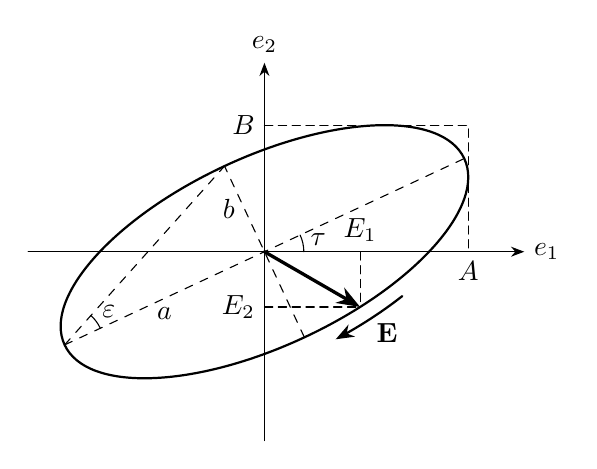
\begin{tikzpicture}[>=Stealth, line cap=round, line join=round, font=\itshape]

  % parameters 
  \def\tilt{25} % tilt angle of the ellipse, tau (deg)
  \def\semiA{2.8}   % semi-major axis length
  \def\semiB{1.2}   % semi-minor axis length
  \def\phiE{-30}    % phase angle of the instantaneous field vector E

  % bounding-box half extents (a_H, a_V)
  \pgfmathsetmacro{\aH}{sqrt((\semiA*cos(\tilt))*(\semiA*cos(\tilt)) + (\semiB*sin(\tilt))*(\semiB*sin(\tilt)))}
  \pgfmathsetmacro{\aV}{sqrt((\semiA*sin(\tilt))*(\semiA*sin(\tilt)) + (\semiB*cos(\tilt))*(\semiB*cos(\tilt)))}

  % point of E on the ellipse boundary, in the lab (x,y) frame
  \pgfmathsetmacro{\rE}{1/sqrt( (cos(\phiE-\tilt)*cos(\phiE-\tilt))/(\semiA*\semiA) + (sin(\phiE-\tilt)*sin(\phiE-\tilt))/(\semiB*\semiB) )}
  \pgfmathsetmacro{\Ex}{\rE*cos(\phiE)}
  \pgfmathsetmacro{\Ey}{\rE*sin(\phiE)}

  % endpoints of the major / minor axis lines (dotted, through the origin)
  \pgfmathsetmacro{\MAx}{\semiA*cos(\tilt)}        % major axis, +tau direction (upper right)
  \pgfmathsetmacro{\MAy}{\semiA*sin(\tilt)}
  \pgfmathsetmacro{\MFx}{\semiA*cos(\tilt+180)}     % major axis, opposite direction (lower left) -> "f"
  \pgfmathsetmacro{\MFy}{\semiA*sin(\tilt+180)}
  \pgfmathsetmacro{\MIx}{\semiB*cos(\tilt+90)}      % minor axis, +90 direction (upper left) -> "e"
  \pgfmathsetmacro{\MIy}{\semiB*sin(\tilt+90)}

  \pgfmathsetmacro{\epsilon}{atan(\semiB/\semiA)}

  % ellipse parameter t0 corresponding to the point (Ex,Ey):
  % rotate (Ex,Ey) back by -tilt into the ellipse's own (u,v) frame,
  % where u = A cos t, v = B sin t
  \pgfmathsetmacro{\uE}{\Ex*cos(\tilt) + \Ey*sin(\tilt)}
  \pgfmathsetmacro{\vE}{-\Ex*sin(\tilt) + \Ey*cos(\tilt)}
  \pgfmathsetmacro{\tE}{atan2(\vE/\semiB, \uE/\semiA)}

  % reference axes 
  \draw[->] (-3,0) -- (3.3,0) node[right]{$e_1$};
  \draw[->] (0,-2.4) -- (0,2.4) node[above] {$e_2$};

  % ellipse 
  \draw[thick] (0,0) ellipse[x radius=\semiA, y radius=\semiB, rotate=\tilt];

  % rotation-direction arrow: short tangential arc at E's own position on the ellipse
  % domain goes from tE+18 down to tE-2 -> arrow points in the *decreasing-t* (clockwise) sense;
  % swap the two domain numbers to flip to counterclockwise
  \draw[->, thick]
    plot[domain={\tE+10}:{\tE-10}, samples=20]
      ({(\semiA + 0.2)*cos(\tilt)*cos(\x) - (\semiB + 0.2)*sin(\tilt)*sin(\x)},
       {(\semiA + 0.2)*sin(\tilt)*cos(\x) + (\semiB + 0.2)*cos(\tilt)*sin(\x)});

  % bounding box (a_H, a_V) 
  \draw[densely dashed] (0,\aV) -- (\aH,\aV) -- (\aH,0);
  \node[left] at (0,\aV) {$B$};
  \node[below] at (\aH,0) {$A$};

  % major / minor axis (dotted) 
  \draw[dashed] (\MFx,\MFy) -- (\MAx,\MAy);
  \draw[dashed] ({-\MIx},{-\MIy}) -- (\MIx,\MIy);
  \node[left] at (\MIx/2,\MIy/2) {$b$};
  \node[below] at (\MFx/2,\MFy/2) {$a$};

  % tilt angle tau 
  \draw (0.5,0) arc[start angle=0, end angle=\tilt, radius=0.5];
  \node at ({\tilt/2}:0.7) {$\tau$};

  % eccentricity
  \draw[dashed] (\MFx,\MFy) -- (\MIx,\MIy);
  \draw (\MFx,\MFy) ++({\tilt}:0.5) arc[start angle=\tilt, end angle={\tilt+\epsilon}, radius=0.5];
  \node at ($(\MFx,\MFy)+({\tilt + \epsilon/2}:0.7)$) {$\varepsilon$};

  % instantaneous field vector E and components 
  \draw[densely dashed] (\Ex,0) -- (\Ex,\Ey);
  \draw[densely dashed] (0,\Ey) -- (\Ex,\Ey);
  \node[above] at (\Ex,0) {$E_1$};
  \node[left] at (0,\Ey) {$E_2$};

  \draw[very thick,->] (0,0) -- (\Ex,\Ey) node[below right, xshift=2pt, yshift=-2pt] {$\mathbf{E}$};

\end{tikzpicture}
\end{document}